\chapter{Evaluating \where~on Test Data}% Main chapter title
\thispagestyle{nohead}
\label{Evaluation} 
%----------------------------------------------------------------------------------------

This chapter will evaluate \where's portfolio algorithm on the held-back test data.
The randomly-selected test set represents 25\% of the entire number of POs and consists of 32 WhyML files, 77 theories and 263 goals  (see Sec. \ref{sub:config}).
In addition to evaluating \where~'s \textit{predictions}, the OCaml implementation (detailed in the previous chapter) will be discussed in terms of its efficiency.   
We perform our evaluation guided by three Evaluation Questions:
\begin{itemize}
	\item[EQ1:] \textbf{How does \where~perform in comparison to the eight SMT solvers?}\\
	The importance of this question is obvious: the success of \where~depends on its improvement over the status quo. In the case of discharging \why~POs, the status quo is represented as the use of a single solver.
	\item[EQ2:] \textbf{How does \where~perform in comparison to the three theoretical strategies?}\\
	The theoretical strategies introduced in Sec. \ref{sec:strategies} provide a fairer basis for comparison than a single solver by taking multiple solver calls per PO into consideration.
	As a reminder for the reader, the \textsf{Best Ranking} always chooses solvers in the order of ascending cost, \textsf{Random Ranking} is the average result of running \textit{every} possible permutation of the eight solvers, and \textsf{Worst Ranking} is the inverse of \textsf{Best Ranking}: it is the ranking of solvers in order of \textit{descending} cost. 
	\item[EQ3:] \textbf{What is the time overhead of using \where~to prove \why~goals?}\\
	The feature extraction and solver scheduling processes incur a time cost. This evaluation criterion measures whether this cost represents a significant proportion of \where~'s overall solving time.    	
\end{itemize}
%The chapter is organised around answering questions raised by each of the three criteria in turn.
This chapter answers each Evaluation Question in turn.
Threats to the validity of our study are discussed in Sec. \ref{sec:threats}. 

\section{EQ1: How does \where~perform in comparison to the eight SMT solvers?}

\label{sec:eq1}

\begin{table}
	\caption[Results for eight solvers, \where~and three strategies on test set]{Number of files, theories and goals proved by each strategy and individual solver. The percentage this represents of the total 32 files, 77 theories, 263 goals, and the average time in seconds, are also shown.}
	\begin{tabularx}{1.1\textwidth}{@{}l|ZZZ|ZZZ|ZZZ@{}}
		\toprule
		{} & \multicolumn{3}{c|}{\textbf{File}} & \multicolumn{3}{c|}{\textbf{Theory}} & \multicolumn{3}{c}{\textbf{Goal}} \\
		{} & \# proved & \% proved & Avg time & \# proved & \% proved & Avg time & \# proved & \% proved & Avg time \\
		\midrule
		\where & 11 & 34.4\% & 1.39 &  44 & 57.1\% & 0.99 & 203 & 77.2\% & 1.98 \\
		\textsf{Best Rank.} & \downbar  & \downbar & 0.25 & \downbar & \downbar & 0.28 & \downbar & \downbar & 0.37 \\
		\textsf{Random Rank.} & \downbar & \downbar & 4.19 & \downbar & \downbar & 4.02 & \downbar & \downbar & 5.70 \\
		\textsf{Worst Rank.} & \upbar & \upbar & 14.71 & \upbar & \upbar & 13.58 & \upbar & \upbar & 18.35 \\
		%\textbf{\textsf{Where4} (tree)} & '' & '' & 4.08 & '' & '' & 2.52 & '' & '' & 3.50 \\
		\midrule
		\textbf{Alt-Ergo-0.95.2} & 8 & 25.0\% & 0.78 & 37 & 48.1\%& 0.26 & 164 & 62.4\% & 0.34 \\ 
		\textbf{Alt-Ergo-1.01} & 10 & 31.3\% & 1.07 & 39 & 50.6\% & 0.26 & 177 & 67.3\% & 0.33 \\ 
		\textbf{CVC3} & 5 & 15.6\% & 0.39 & 36 & 46.8\% & 0.21 & 167 & 63.5\% & 0.38 \\ 
		\textbf{CVC4} & 4  & 12.5\% & 0.56 & 32 & 41.6\% & 0.21 & 147 & 55.9\% & 0.35 \\ 
		\textbf{veriT} & 2 & 6.3\% & 0.12 & 24 & 31.2\% & 0.12 & 100 & 38.0\% & 0.27 \\ 
		\textbf{Yices} & 4 & 12.5\% & 0.32 & 32 & 41.6\% & 0.15 & 113 & 43.0\% & 0.18 \\ 
		\textbf{Z3-4.3.2} & 6 & 18.8\% & 0.46 & 31 & 40.3\% & 0.20 & 145 & 55.1\% & 0.37 \\ 
		\textbf{Z3-4.4.1} & 6 & 18.8\% & 0.56 & 31 & 40.3\% & 0.23 & 145 & 55.1\% & 0.38 \\ 
		\bottomrule
	\end{tabularx}
	\label{table:avgtimes2}
\end{table}

\begin{figure}
	\centering
	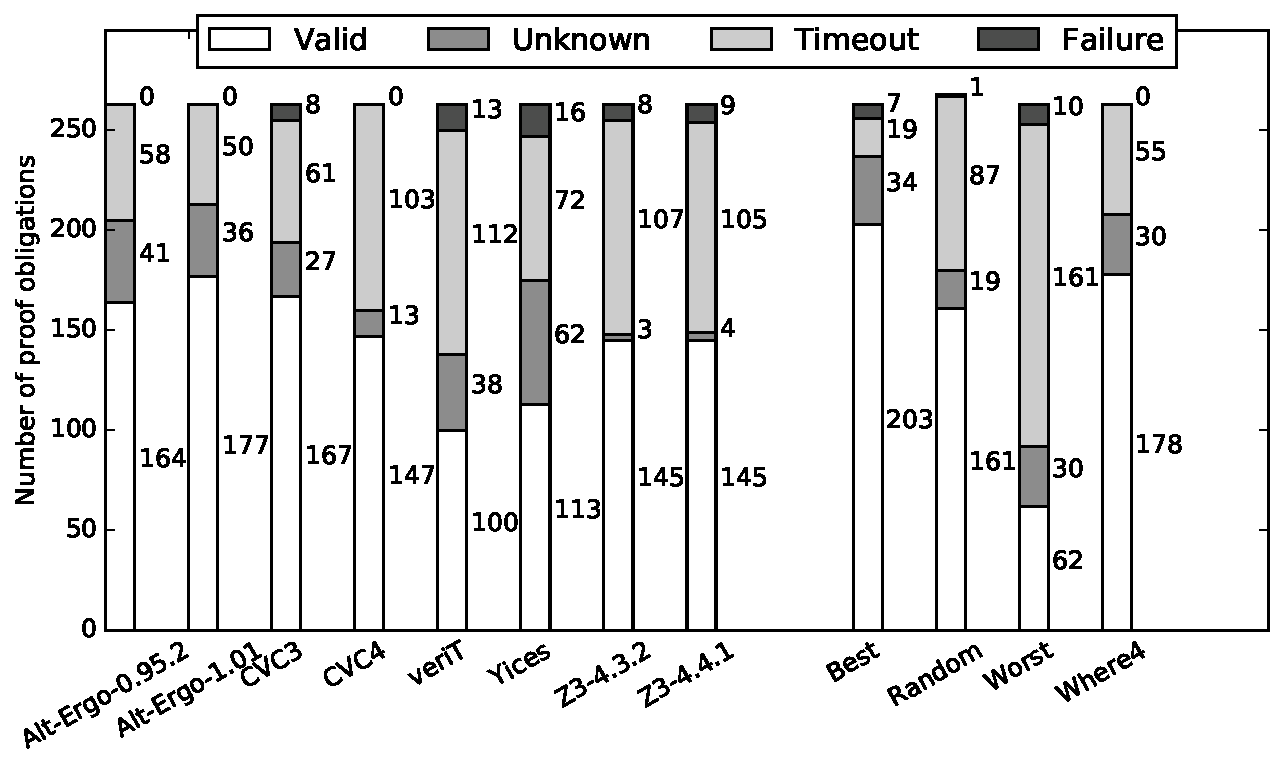
\includegraphics[width=\linewidth]{barcharts2}
	\caption[The relative amount of Valid/Unknown/Timeout/Failure answers from the eight SMT solvers, \where, and three theoretical strategies.]{The relative amount of Valid/Unknown/Timeout/Failure answers from the eight SMT solvers, \where~(pre-solver = Alt-Ergo-1.01), and three theoretical strategies on the 263 test POs (with a timeout limit of ten seconds).}
	\label{fig:barchart2}
\end{figure}


When each solver in \textsf{Where4}'s ranking sequence is run on each goal, the maximum amount of files, theories and goals are provable. 
As previously mentioned in Sec. \ref{sub:worst} and as Table \ref{table:avgtimes2} shows, the difference between \where~and the set of reference theoretical strategies (\textsf{Best Ranking}, \textsf{Random Ranking}, and \textsf{Worst Ranking}) is the amount of time taken to return the \textit{Valid/Invalid} result. 
Compared to the eight SMT solvers, the biggest increase is on individual goals: \textsf{Where4} can prove 203 goals, which is 26 (9.9\%) more goals than the next best single SMT solver, Alt-Ergo-1.01.

As is shown by Table \ref{table:avgtimes2}, the average time taken for \textsf{Best Ranking} to return an answer of \textit{Valid} is not necessarily less than that of an individual solver. 
As \textsf{Best Ranking} can return \textit{Valid} for all provable POs -- more than any individual solver --
it is the number of \textit{Valid} answers, rather than any inefficiency, that is responsible for this slightly slower average time.  

The average time \where~takes to prove these goals 
(using Algorithm \ref{algo:where4}) 
is significantly better than the \textsf{Random Ranking} strategy.
It is, however, lagging behind the time recorded by the \textsf{Best Ranking} strategy. 

In comparison to the eight SMT solvers, the average time taken by \where~to prove each of the 203 goals is high. 
This tells us that \where~can perform badly with goals which are not provable by many SMT solvers: expensive \textit{Timeout} results are chosen before the \textit{Valid} result is eventually returned. 
In the worst case, \where~may try all eight solvers in sequence, timing out for each solver, whereas each individual solver does this just once. 
Thus, while having access to more solvers can allow more goals to be proved (if there are goals uniquely-provable by the solvers such as those identified in Table \ref{table:unique}), there is also a time penalty associated with portfolio-based solvers in these circumstances.
This issue has previously been identified by Amadini et al. in their studies on portfolio solvers for constraint programming \cite{Amadini2013} and constraint optimisation \cite{Amadini2016} where portfolio performance was found to degrade as the number of constituent solvers increased.

The multiple timeout issue raises the question of whether it is fair to compare \where~to individual solvers. 
Any ranking strategy will be able to prove the maximum number of files, theories and goals, but unless the best solver is consistently placed high in the ranking, it could take a significantly longer time to do so than even the worst-performing individual solver.   

We remind the reader of the \textsf{Choose Single} solver introduced in Sec. \ref{sec:portfolio-benefit}.
\textsf{Choose Single} is the \textit{best single solver} as chosen on a per-goal basis.
It provided a motivation for the use of portfolio-solving on the \why~platform by proving the maximum number of goals in the shortest amount of time.
We mentioned that \textsf{Choose Single} is equivalent to choosing  the top-ranking solver from \textsf{Best Ranking} and stopping.
We return to this concept in Fig. \ref{fig:barchart2} which is similar to Fig. \ref{fig:barcharts} in that it shows the relative amount of Valid/Unknown/Timeout/Failure answers from the eight SMT solvers. 
Also shown (on the right) are results obtainable by using the top solver (only) with the three ranking strategies (where \textsf{Best Ranking} $\equiv$ \textsf{Choose Single}) and the \where~predicted ranking (after pre-solving with Alt-Ergo version 1.01).


\begin{algorithm}
	\caption{Returning answers and runtimes from \where~solver rankings using a cost threshold: A minor modification to Alg. \ref{algo:where4} with an additional stopping condition in the \textbf{while} loop}
	\KwIn{$P$, a \why~program;\\ 
		$R$, a static ranking of solvers for pre-proving; \\
		$\phi$, a timeout value; \\ 
		$\mu$, the cost threshold}
	\KwOut{$\langle A,T\rangle$ where \\
		$A$ = the best answer from the solvers; \\
		$T$ = the cumulative time taken to return $A$}
	\Begin{
		\tcc{pre-solving}
		$S \leftarrow BestInstalled(R) $ \\				
		$\langle A,T \rangle \leftarrow Call(P, S, 1)$ \\
		\If{$A \in \lbrace Valid, Invalid \rbrace $}
		{\Return{$\langle A,T \rangle$}}
		$F \leftarrow ExtractFeatures(P) $ \\
		$R \leftarrow PredictRanking(F) $ \\
		\tcc{the predicted cost of $S$ is an additional stopping condition}
		\While{$A \notin \lbrace Valid, Invalid \rbrace \wedge R \neq \emptyset \wedge Cost(S) \leq \mu$}
		{$S \leftarrow BestInstalled(R) $ \\	
			$\langle A_S,T_S \rangle \leftarrow Call(P, S, \phi)$ \\
			$T \leftarrow T + T_S$  \\
			\If{$A_S > A$}
			{	
				$A \leftarrow A_S$ }
			\tcc{remove $S$ from the set of solvers $R$}
			$R \leftarrow R \setminus \lbrace S \rbrace$}
		\Return{$\langle A,T\rangle$}}
	\label{algo:threshold}
	
\end{algorithm}

The 62 \text{Valid} answers returned by the top solver from the \textsf{Worst Ranking} (i.e. the worst solver) represent the trivial POs solvable by all eight solvers. 
Likewise, the 60 goals for which \textsf{Best Ranking} did not return a \textit{Valid} or \textit{Invalid} answer could not be proved by any solver.

The results show that limiting the portfolio solver to just using the best predicted individual solver eliminates the multiple time-out overhead yet reduces the number of goals provable by \where.
This number of goals -- 184 -- is still more than the best-performing individual SMT solver, Alt-Ergo version 1.01.  

In an effort to compare \where~to individual SMT solvers, Table \ref{table:avgtimes2} and Fig. \ref{fig:barchart2} show results at two extremes of a spectrum: using all solvers available, and only using one.
In the next subsection we describe a method to calibrate the use of \where~by using the predicted cost of each solver. 


\subsection{Use of a cost threshold}
\label{sub:threshold}

To balance the time-taken-versus-goals-proved trade-off associated with the two approaches above, we introduce the notion of a \textit{cost threshold} as another method of comparing \where~to individual SMT solvers.
\where's use of a cost threshold constitutes a minor adjustment to Alg. \ref{algo:where4} and is detailed in Alg. \ref{algo:threshold}. 
After pre-solving, solvers with a predicted cost above this threshold are not called. 
If every solver's cost is predicted to be above the threshold $\mu$, the pre-solver's result is returned.
%This modification to Algorithm \ref{algo:where4} is shown in Algorithm \ref{algo:threshold}    

We determine the appropriate value for this threshold by first splitting the training data into model training and validation sets.
The model training set used for this step represents 90\% of the total training set (or 706 POs), while the validation set is made up of 79 POs. 
We train the Random Forest predictor (with pre-solving) before simulating the effect of an increasing cost threshold using the validation set.

\begin{figure}
	\centering
	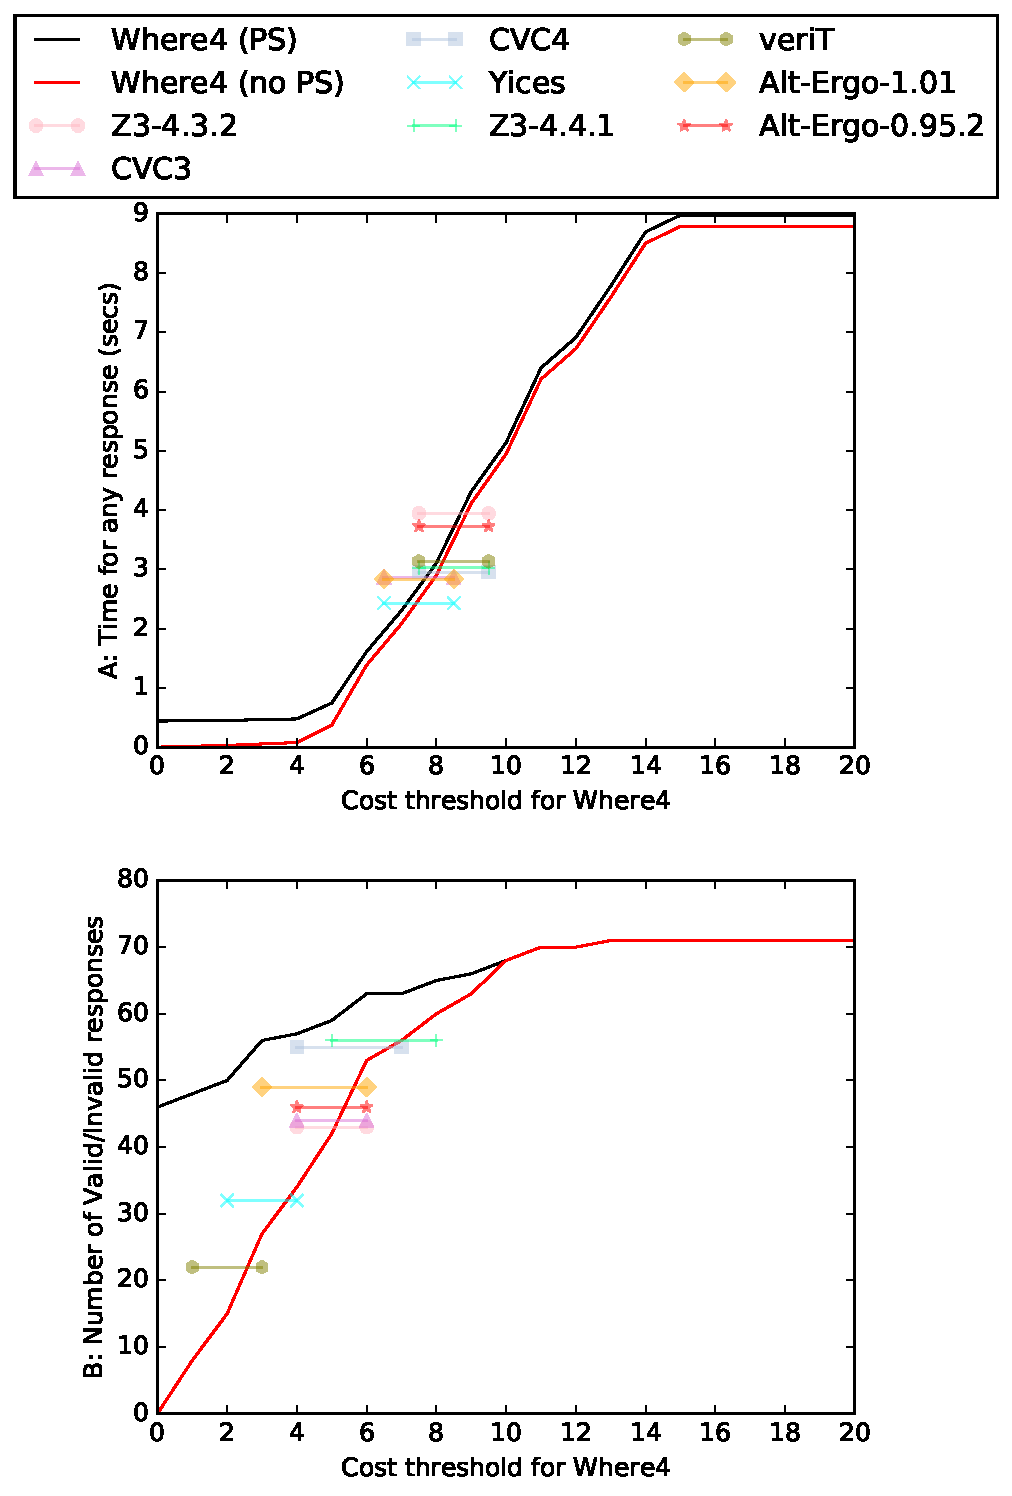
\includegraphics[width=\linewidth]{thresholds1}
	\caption[Determining a cost threshold]{Determining the appropriate value for a cost threshold (using a validation dataset). (\textit{a: top plot}) The average time taken for \where~to return an answer compared to eight SMT solvers. (\textit{b: bottom plot}) The number of Valid/Invalid answers returned by \where~compared to eight SMT solvers.}
	\label{fig:thresholds1}
\end{figure}  


\begin{figure}
	\centering
	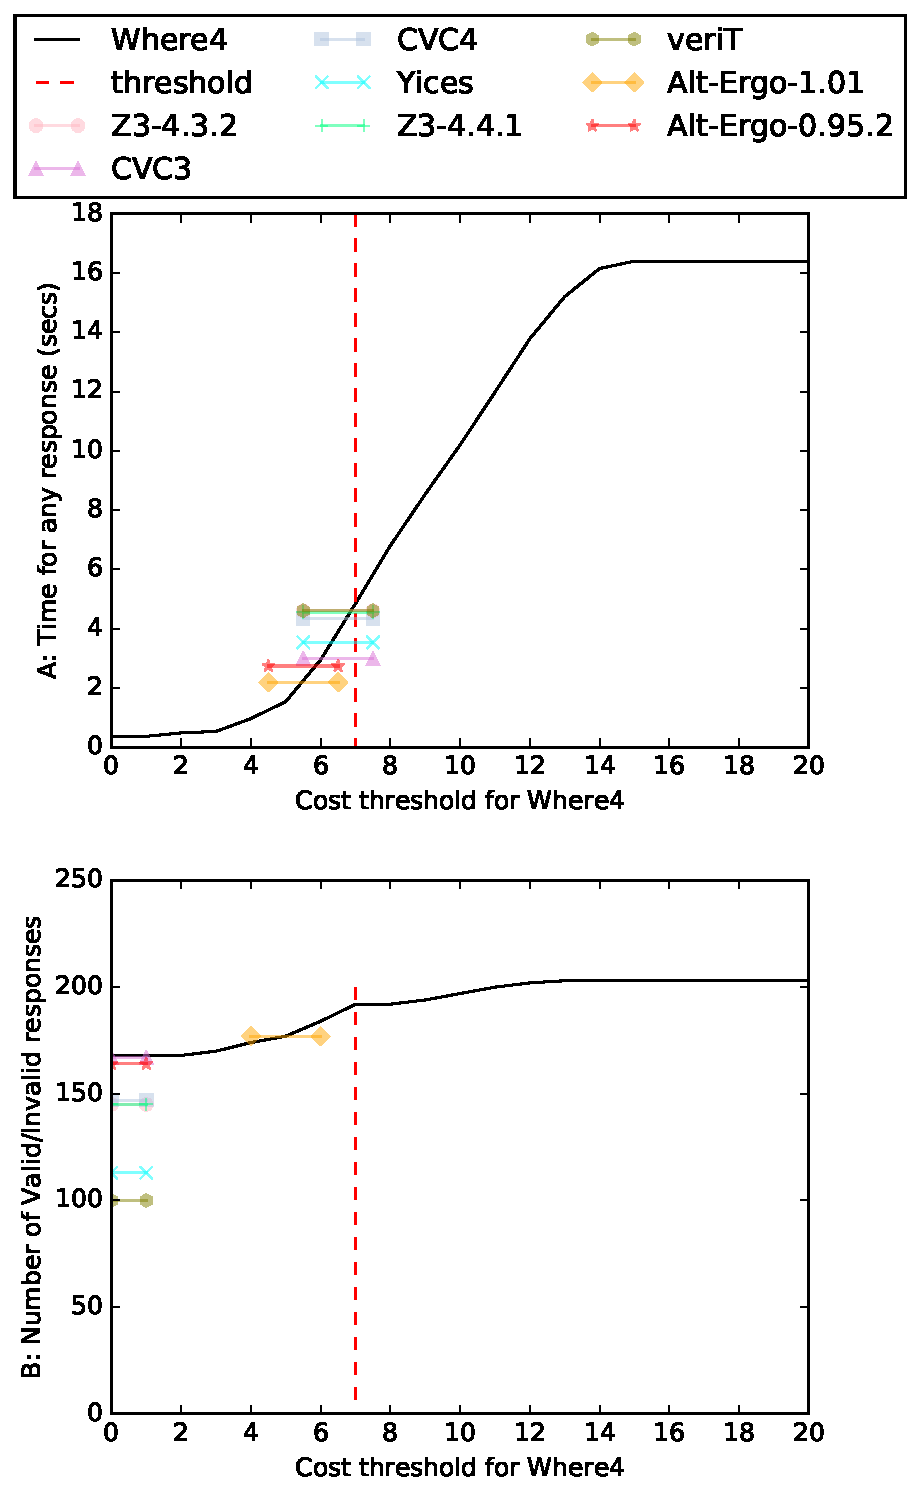
\includegraphics[width=\linewidth]{thresholds2}
	\caption[The effect of using a cost threshold]{The effect of using a cost threshold. (\textit{a: top plot}) The average time taken for \where~to return an answer compared to eight SMT solvers. (\textit{b: bottom plot}) The number of Valid/Invalid answers returned by \where~compared to eight SMT solvers.}
	\label{fig:thresholds2}
\end{figure}



Fig. \ref{fig:thresholds1}a and \ref{fig:thresholds1}b show the effect of varying this threshold when solving POs in the test set.
The top plot (\textit{a}) shows a comparison of the average time taken for \textit{any} answer to be returned (not necessarily \textit{Valid / Invalid}).
The amount of time taken by \where~often depends on the number of solvers called.
The number of solvers called depends on the cost threshold given to \where. 
The solid black line of Fig. \ref{fig:thresholds1}a, shows the increase in average time taken by \where~to return a response as the cost threshold increases.
Fig. \ref{fig:thresholds1}b shows the number of \textit{Valid / Invalid} responses returned by each individual SMT solver as compared to \where~with a range of threshold values.
As the corresponding results for each individual solver are unaffected by the threshold parameter, they are represented by horizontal line segments intersecting with the \where~data in Fig. \ref{fig:thresholds1}a.

We note that even when given a threshold value of zero, 46 POs are proven.
The pre-solving routine (in our case, Alt-Ergo-1.01 given a time limit of one second) is responsible for these results (as the solver cost is never used).
As this figure is larger than the number of provable goals for all but three individual solvers, their results are shown as horizontal lines on the left side of the y-axis.
As in Fig. \ref{fig:thresholds1}a, the results for each individual solver are unaffected by the threshold parameter.

By inspecting these results, we find that a threshold value of seven gives good results.
At this threshold, far more \textit{Valid/Invalid} are returned than the best-performing individual solver (Z3-4.4.1) and they are returned in a faster time (on average) than the fastest-returning solver (Yices).

As the dashed red line in Fig. \ref{fig:thresholds2} shows, a threshold value of seven also performs well on the test data.
These results are shown in numerical form in Table \ref{table:threshold}. 
When \where~is given a cost threshold of five, it can prove the same number of POs as the best-performing solver -- Alt-Ergo-1.01. 
By referring to Fig. \ref{fig:thresholds2}a, we see that at the same cost threshold, it takes a shorter time to return a response, on average, than the fastest SMT solver (which is also Alt-Ergo-1.01).
If the cost threshold is increased to seven, significantly more POs can be proven. 
The average time taken to return a response is approximately equal to that of the four slowest individual solvers on the test data: CVC4, veriT, and both versions of Z3. \\
\\
\textbf{EQ1 Answer:} The cost threshold greatly improves \where's performance in comparison to the individual SMT solvers.
The performance penalties associated with portfolio solvers can be mitigated by defining a cut-off point and trusting that solvers with a predicted cost greater than this value do not need to be called.
We found this point to be about seven for the POs in the \textsf{Why3} example dataset.
The value to choose as a threshold may not be obvious in real-world scenarios with unseen results, however. 


\begin{table}
	\caption[The effect of using a cost threshold]{The effect of using a cost threshold. The average time taken for \where~to return an answer compared and the number of Valid/Invalid answers. Same data as Fig. \ref{fig:thresholds2}}
	\begin{tabularx}{0.9\textwidth}{@{}l|Z|Z|Z|Z|Z|Z@{}}

		\textsc{Threshold} & \textbf{0} & \textbf{1} & \textbf{2} & \textbf{3} & \textbf{4} & \textbf{5} \\
		\midrule
		\textbf{Avg. Time} & 0.37 & 0.37 & 0.48 & 0.53 & 0.98 & 1.77  \\
		\textbf{Num. Proved} & 168 & 168 & 168 & 169 & 173 & 177  \\
		\midrule
		\midrule
		\textsc{Threshold}  & \textbf{6} & \textbf{7} & \textbf{8} & \textbf{9} & \textbf{10} & \textbf{11}  \\
		\midrule
		\textbf{Avg. Time} & 2.72 & 4.59 & 6.55 & 8.74 & 10.31 & 11.89  \\
		\textbf{Num. Proved} & 183 & 192 & 192 & 195 & 197 & 199 \\
		\midrule
		\midrule
		\textsc{Threshold} & \textbf{12} & \textbf{13} & \textbf{14} & \textbf{15} & \textbf{16} & \textbf{17} \\
		\midrule
		\textbf{Avg. Time} & 14.16 & 15.24 & 16.06 & 16.35 & 16.35 & 16.35 \\
		\textbf{Num. Proved}  & 202 & 203 & 203 & 203 & 203 & 203 \\
		
	\end{tabularx}
	\label{table:threshold}
\end{table}

\section{EQ2: How does \where~perform in comparison to the three theoretical strategies?}


\begin{figure}
	\centering
	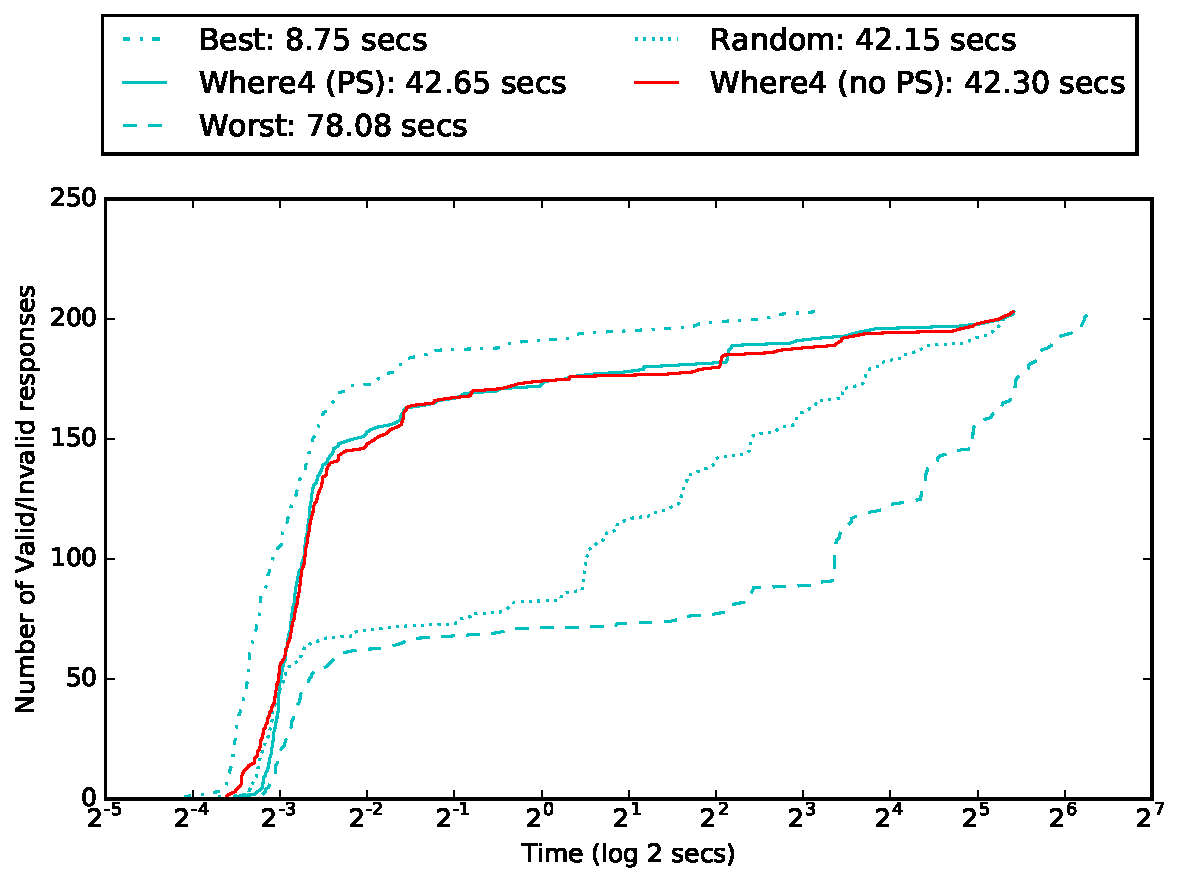
\includegraphics[width=1.0\linewidth]{line_graph_eval_provers}
	\caption{The time taken by each theoretical strategy and \where~to return all \textit{Valid/Invalid} answers in the test dataset of 263 goals}
	\label{fig:line_graph_eval_provers}
\end{figure}

Fig. \ref{fig:line_graph_eval_provers} compares the time taken for \where~and the three ranking strategies to return \textit{Valid} answers for the 263 POs in the test set.
This experiment is equivalent to running each strategy on all 263 POs in parallel and measuring the time taken for each strategy to return a total of 203 \textit{Valid} answers.
As described in Sec. \ref{sec:strategies}, \textsf{Best Ranking} and \textsf{Worst Ranking} use Alg. \ref{algo:rank} to return their time taken.
\textsf{Random Ranking}'s time measurement is based on the average of 40,320 (i.e. eight factorial, the number of individual rankings) uses of Alg. \ref{algo:rank}.
\where's times are derived from the use of Alg. \ref{algo:where4} with a pre-solver of Alt-Ergo-1.01. 
Although both \where~and \textsf{Random Ranking} finish at approximately the same time, \where~is significantly faster for returning \textit{Valid/Invalid} answers. 
\where's solid line is more closely correlated to \textsf{Best Ranking}'s rate of success than the erratic rate of the \textsf{Random Ranking} strategy. 
Again, we find that \where~struggles to prove a small number of POs.
\textsf{Best Ranking}'s excellent time result shows the capability of a perfect-scoring learning strategy. \\
\\
\textbf{EQ2 Answer:} At almost any point in time from zero seconds to 42.65 seconds, the number of \textit{Valid/Invalid} answers returned by \where~is greater than the number returned by \textsf{Random Ranking}.
This shows that our prediction model is a better choice than selecting a sequence of SMT solvers at random, without any regard to program features or solver capability.
\where's performance on all but the hardest POs is encouraging.
Although \where~cannot compete with \textsf{Best Ranking} yet, the performance of this theoretical strategy is motivation to further improve \where~in the future.   



\section{EQ3: What is the time overhead of using \where~to prove \why~goals?}

\label{sec:eq3}

The timings for \where~in all plots and tables in this chapter are based solely on the performance of the constituent solvers (the measurement of which is discussed in Sec. \ref{sec:dependant}). They do not measure the time it takes for the OCaml binary to extract the static metrics, traverse the decision trees and predict the ranking. 
We have found that this adds (on average) 0.46 seconds to the time \where~takes to return a result for each of the files in the test set. 
On a per goal basis, this is equivalent to an increase in 0.056 seconds.
This overhead is only applied to goals for which pre-solving is unsuccessful.  
For the test set, pre-solving eliminated this overhead for 168 out of 263 POs (see Table \ref{table:threshold}: \where's number of \textit{Valid/Invalid} responses when the cost threshold is zero).

The imitation of an orthodox solver to interact with \why~is more costly: this is due to \why~printing each goal as a temporary file to be read in by the solver individually (see Sec. \ref{sec:why3-integration}). 
As \where~uses the abstract, internal representation of the program, the printing of each goal to the Why format is unnecessary.
The \why~driver mechanism makes this step unavoidable for any supported solver including, of course, the \where~``imitation solver''.

Another issue with calling \where~through \why~is that of applying \why's timeout value to a sequence of solver calls. 
For example, if a user gives \why~a timeout of five seconds for \where~to prove a PO and the first solver called by \where~goes over that limit, the potentially useful answer returned by the second solver in the sequence would not be returned to the user. \\
\\
\textbf{EQ3 Answer:}
While pre-solving is an important heuristic for avoiding the overhead of feature extraction and rank prediction, these processes must be optimised for \where~to be practical as a portfolio solver called from \why.   
Future work will look at a portfolio-solving \why~plugin similar to \where. Tighter integration with the \why~system can be expected to improve the efficiency of such a tool.      
In its current form, \where~is more suited to an initial proving step performed using the stand-alone command line tool.

\section{Threats to Validity}
\label{sec:threats}

In this section we discuss the threats to the validity of the evaluation presented in this chapter.
We categorise threats as either \textit{internal} or \textit{external}.
Internal threats refer to influences that can affect the response variable without the researcher's knowledge and threaten the conclusions reached about the \textit{cause} of the experimental results \cite{experimentation}. 
Threats to external validity are conditions that limit the generalisability and reproducibility of an experiment. 

\subsection{Internal}

The main threat to our work's internal validity is selection bias. All of our training and test samples are taken from the same source. 
We took care to split the data for training and testing purposes on a \textit{per file} basis, as we discussed in Sec. \ref{sub:config}. 
This ensured that \where~was not trained on a goal belonging to the same theory or file as any goal used for testing.
 
The results of running the solvers on our dataset are imbalanced. There were far more \textit{Valid} responses than any other response. 
No goal in our dataset returned an answer of \textit{Invalid} on any of the eight solvers. 
This is a serious problem as \where~would not be able to recognize such a goal in real-world use. 

Use of an independent dataset is likely to influence the performance of the solvers. 
Alt-Ergo was designed for use with the \why~platform -- its input language is a previous version of the Why logic language. 
It is natural that the developers of the \why~examples would write programs which Alt-Ergo in particular would be able to prove. 
Due to the syntactic similarities in input format and logical similarities such as support for type polymorphism, it is likely that Alt-Ergo would perform well with any \why~dataset. We would hope, however, that the gulf between it and other solvers would narrow.

There may be confounding effects in a solver's results that are not related to the independent variables we used (Sec. \ref{sec:independant}). 
We were limited in the tools available to extract features from the domain-specific Why logic language (in contrast to related work on model checkers which use the general-purpose C language \cite{DPVZ15:CAV, MUX} -- as previously discussed in Sec. \ref{sub:lrsvmmml}). 
We made the decision to keep the choice of independent variables simple in order to increase generalisability to other formalisms such as Microsoft's Boogie \cite{Boogie} intermediate language.  

\subsection{External}


The generalisability of our results is limited by the fact that all dependent variables were measured on a single machine.
All data collection was conducted on a single 64-bit machine running Ubuntu 14.04 with a dual-core Intel i5-4250U CPU and 16GB of RAM. 
We believe that the number of each response for each solver would not vary dramatically on a different machine of similar specifications. 
By inspecting the results when each solver was given a timeout of 60 seconds (Fig. \ref{fig:line_graph}), the rate of increase for \textit{Valid/Invalid} results was much lower than that of \textit{Unknown/Failure} results. 
The former set of results are more important when computing the cost value for each solver-goal pair.

Timings of individual goals are likely to vary widely (even across independent executions on the same machine).
% Locally, we used a statistically-accurate mean timing based on a 90\% confidence interval (see Sec. \ref{sec:dependant}). 
It is our assumption that although the actual timed values would be quite different on any other machine, the \textit{ranking} of their timings would stay relatively stable.

A ``typical'' software development scenario might involve a user verifying a single file with a small number of resultant goals: certainly much smaller than the size of our test set (263 goals). In such a setting, the productivity gains associated with using \where~would be minor. 
\where~is more suited therefore to large-scale software verification.


\section{Discussion}
\label{sec:eval-discuss}

By considering the answers to our three Evaluation Questions, we can make assertions about the success of  \where.
The answer to \textbf{EC1}, \where's performance in comparison to individual SMT solvers, is positive.
A small improvement in \textit{Valid/Invalid} responses results from using only the top-ranked solver, while a much bigger increase can be seen by making the full ranking of solvers available for use.
The time penalty associated with calling a number of solvers on an un-provable PO is mitigated by the use of a \textit{cost threshold}.
Judicious use of this threshold value can balance the time-taken-versus-goals-proved trade-off: in our test set of 263 POs, using a threshold value of seven results in 192 \textit{Valid} responses -- an increase of fifteen over the single best solver -- in a reasonable average time per PO (both \textit{Valid} and otherwise) of 4.59 seconds.

There is also cause for optimism in \where's performance as compared to the three theoretical ranking strategies -- the subject of Evaluation Question 2. 
All but the most stubborn of \textit{Valid} answers are returned in a time far better than \textsf{Random Ranking}.
We take this random strategy as representing the behaviour of the non-expert \why~user who does not have a preference amongst the variety of supported SMT solvers.
For this user, \where~could be a valuable tool in the efficient initial verification of POs through the \why~system.    

In terms of time overhead -- the concern of EQ3 -- our results are less favourable, particularly when \where~is used as an integrated part of the \why~toolchain.
The costly printing and parsing of POs slows \where~beyond the time overhead associated with feature extraction and prediction.
At present, due to the diversity of languages and input formats in use for SV (see Sec. \ref{sec:lrsv}), this is an unavoidable pre-processing step enforced by \why~(and is indeed one of the \why~system's major advantages).

Overall, we believe that the results for two out of three Evaluation Questions are encouraging and suggest a number of directions for future work to improve \where.
 

 

